\documentclass[11pt, oneside, a4paper]{book}

\usepackage{fancyhdr}
\pagestyle{fancy}
\fancyhf{}

\usepackage[english]{babel}
\usepackage{graphicx}
\usepackage[colorlinks,hyperindex,plainpages=false,breaklinks]{hyperref}
\usepackage{amssymb}
\usepackage{wasysym} 
\usepackage{wrapfig}
\usepackage{enumerate}
\usepackage{placeins} % Necessary for \FloatBarrier
\usepackage{subfig}   % Necessary for subfloat (images next to each other)
\usepackage{color}
\usepackage[usenames,dvipsnames,svgnames]{xcolor}
\usepackage{listings}
\usepackage{fancyhdr}

\definecolor{codelightgray}{rgb}{0.87,0.87,0.87}

\hypersetup{colorlinks=true,% 
	linkcolor=black,%
	citecolor=red,%
	filecolor=blue,% 
	menucolor=black,% 
	pagecolor=black,%
	urlcolor=black}
	
\lstset{language=,
    keywordstyle=\color{blue},
    basicstyle=\scriptsize\ttfamily,
    showstringspaces=false,
    backgroundcolor=\color{codelightgray},
    morekeywords={SELECT,FROM,WHERE,AND,OR,EClass}
}

% Set TOC depth
\setcounter{tocdepth}{2}

\setlength{\parindent}{0pt} 
\setlength{\parskip}{0.3cm}

\graphicspath{{../introduction_images/}{../../06_miscellaneous/commonFiles/}}

% --- HEADER FUNCTIONS % --------------------------------------------------------------------------------------------------------------------------------------
% Default plain header; turn off all lines and colors; turn on page numbers for all headers
\newcommand{\noHeader}{
 	\fancyhead[OR]{\thepage}
	\fancyhead[OL]{}
 	\fancyhead[EL]{\thepage}
	\fancyhead[ER]{}
	\renewcommand{\headrulewidth}{0pt}
}

% Common instruction Header; Black
\newcommand{\genHeader}{
	\fancyhead[OL]{}
	\fancyhead[ER]{}
	\renewcommand{\headrulewidth}{1.5pt}
 	\renewcommand{\headrule}{\hbox to\headwidth{%
  		\color{Black}\leaders\hrule height \headrulewidth\hfill}}
}
% -------------------------------------------------------------------------------------------------------------------------------------------------------------

% TODO:  Set individual handbook download links (appears on description page)
% Custom links created at: http://tinyurl.com/
\newcommand{\rootLink}[1]{\url{http://tinyurl.com/emoflon-docs/#1}}
\newcommand{\dlPartOne}{\rootLink{part1.pdf}}
\newcommand{\dlPartTwo}{\rootLink{part2.pdf}}
\newcommand{\dlPartThree}{\rootLink{part3.pdf}}
\newcommand{\dlPartFour}{\rootLink{part4.pdf}}
\newcommand{\dlPartFive}{\rootLink{part5.pdf}}
\newcommand{\dlPartSix}{\rootLink{part6.pdf}}

% TODO:	Set time it takes to complete each part
\newcommand{\timeTwo}{1h}
\newcommand{\timeThree}{3h}
\newcommand{\timeFour}{1h 30min}
\newcommand{\timeFive}{2h}
\newcommand{\timeSix}{30 min}

% TODO:  Update version number (Title Page Information)
\def\partTitle{Part 0: Introduction}
\def\versionNumber{0.1} 
\title{
\flushright
{\LARGE\bfseries An Introduction to Metamodelling\\
and Graph Transformations}
\noindent\rule[-1ex]{\textwidth}{5pt}\\[2.5ex]
\hfill\emph{\LARGE\bfseries with eMoflon}
\flushleft
{\small Version 2.1}
\flushright

\includegraphics[width=0.85\textwidth]{pics/eMoflon3} 
}

\date{}  
\author{} 
% -------------------------------------------------------------------------------------------------------------------------------------------------------------

\begin{document}

\frontmatter
\noHeader

% Title Page without trailing blank page
{\let\newpage\relax\maketitle}

% Copyright notice
\begin{small} 
Copyright \copyright~2011--\the\year{} Real-Time Systems Lab, TU Darmstadt.
Anthony Anjorin, Erika Burdon, Frederik Deckwerth, Roland Kluge, Marius Lauder,
Erhan Leblebici, Daniel T\"ogel, David Marx, Lars Patzina, Sven Patzina, Alexander Schleich, Sascha Edwin Zander, Jerome Reinl\"ander, Martin Wieber, and contributors.
All rights reserved.

This document is free; you can redistribute it and/or modify it under the terms of the GNU Free Documentation License as published by the Free Software Foundation; either version 1.3 of the License, or (at your option) any later version.
Please visit \href{http://www.gnu.org/copyleft/fdl.html}{http://www.gnu.org/copyleft/fdl.html} to find the full text of the license.
 
% TODO Remove this?? It can be found easily online .. (we can even offer it on
% the download page) For your convenience, this document includes a copy of the \emph{GNU General Public License} starting from page~\pageref{chap:gpl}.
  
For further information contact us at \eMoflonContact.
  
\vskip3cm
\textit{The eMoflon team}\\
Darmstadt, Germany (\monthword{\month} \the\year)
\end{small}
\let\cleardoublepage\clearpage

% Store page counter
\newcounter{romanpages}
\setcounter{romanpages}{\value{page}}

\mainmatter

% Main content for this part
\genHeader

{\bf \huge Part 0:}

\vspace{0.8cm}

{\bf \Huge Introduction }

\vspace{2cm}


This handbook has been engineered to be \emph{fun}.

If you work through it and, for some reason, do \emph{not} have a resounding \mbox{``I-Rule''} feeling afterwards, please send us an email and tell us how to
improve at \href{mailto:contact@moflon.org}{contact@moflon.org} .

\begin{figure}[htp]
\begin{center}
	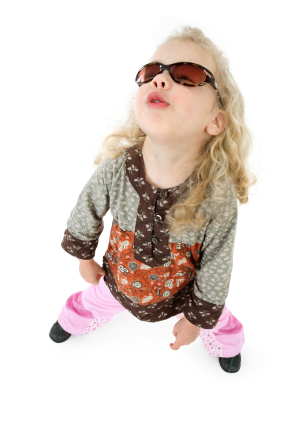
\includegraphics[height=0.45\textheight]{../introduction_images/i-rule}
	\caption{How you should feel when you're done}
	\label{i-rule}
\end{center}
\end{figure}
\break
 

To enjoy the experience, you should be fairly comfortable with Java or a comparable object-oriented language, and know how to perform basic tasks in Eclipse. 
Although we assume this, we give references to help bring you up to speed as necessary. Last but not least, basic knowledge of common UML notation would be
helpful.

Our goal is to give a \emph{hands-on} introduction to metamodelling and graph transformations using our tool \emph{eMoflon}. The idea is to \emph{learn by
doing} and all concepts are introduced while working on a concrete example. The language and style used throughout is intentionally relaxed and non-academic.


{\bf \large So, what is eMoflon?}

eMoflon is a tool for building tools. If you wish, a ``meta" tool.  This means that if you're interested in building \emph{domain specific} tools for end users,
then eMoflon could be pretty useful for you.


{\bf \large Why should I be interested?}

To build a tool, you typically need a way for users to communicate with it, i.e., you must establish a suitable \emph{language} for specifying input and output
to and from the tool.  You also need a central data structure to represent the ``state" of the tool.  This data structure or \emph{model} is usually manipulated
and appropriately \emph{transformed} in some useful manner by the tool.  Many tools also \emph{generate} something useful from their internal models and keep
them synchronized with other models in different tools. To achieve these goals you can use \emph{metamodelling} to define your language (your \emph{meta}model),
\emph{graph transformations} to transform your models, and parsing/code generation techniques to produce something useful from your models. All this and much
more is supported by eMoflon. Take a look at Fig.~\ref{fig:transModel} to see how all these tasks fit together.

{\bf \large What does this handbook cover?}

On the last page, we've described each of the 6 parts that make up this handbook. You can work through them sequentially and become an
\emph{official}\footnote{Certificate not guaranteed} eMoflon master or, depending on your interests, decide what you'd like to read and what to skip. We
provide all the necessary materials (i.e., a cheat package) so you can jump right in without having to complete the previous parts. For those of you interested
in further details and the mature formalism of graph transformations, we give relevant references throughout the handbook.

\vfill \newpage

\vspace*{2cm}
\begin{figure}[htbp]
	\centering
  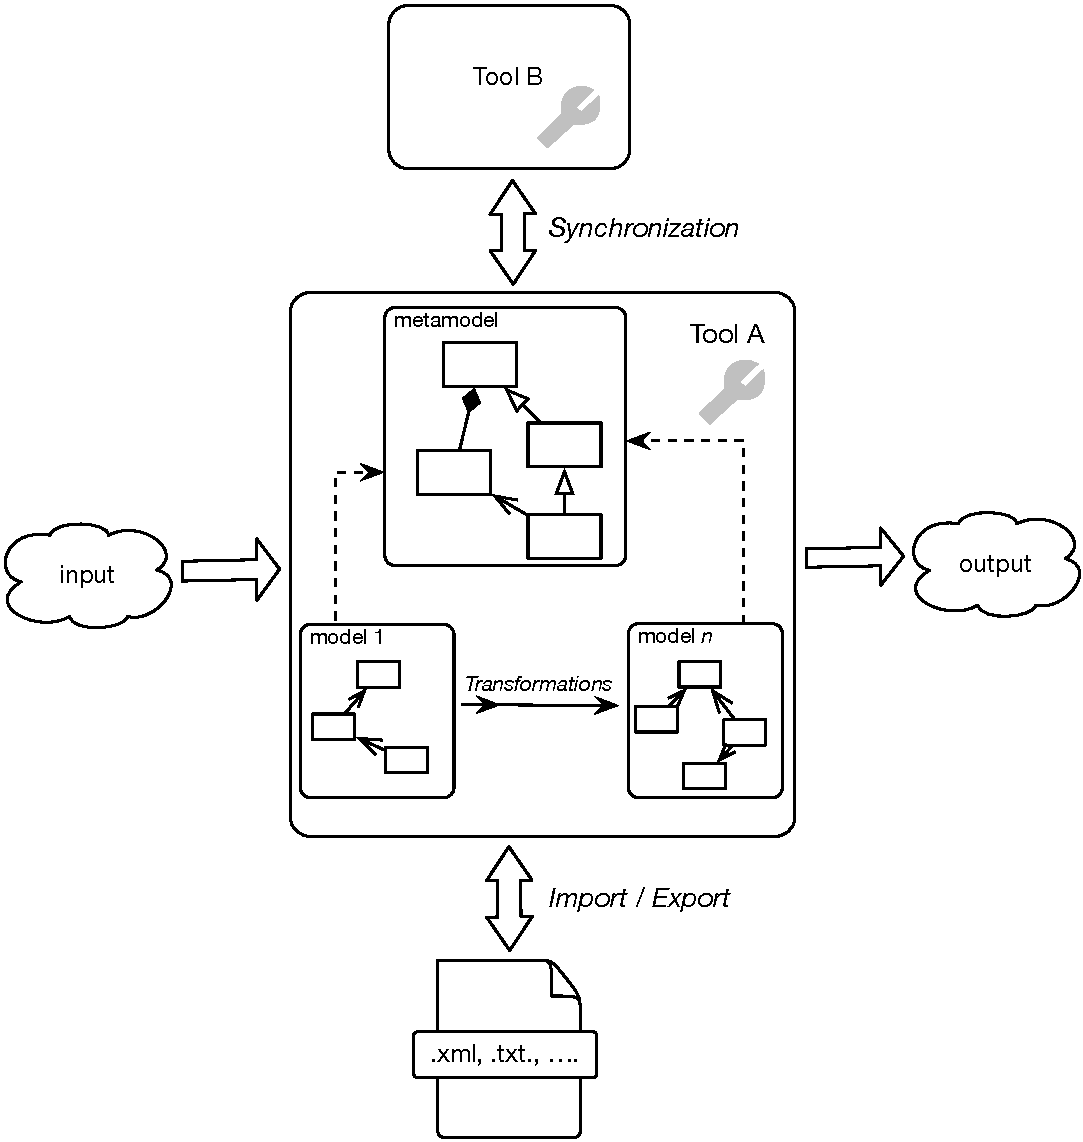
\includegraphics[width=0.9\textwidth]{eMoflonDiagram.pdf}
	\caption{Building a tool requires language specification (metamodelling), transformations, synchronization, parsing, and code generation}
	\label{fig:transModel}
\end{figure}
\begin{description}

\pagebreak

\item[Part I: Installation and Set Up] provides a very simple example and a few JUnit tests to test the installation and configuration of eMoflon. We also
explain the general workflow and the different workspaces involved.

This part can be considered \emph{mandatory} only if you are new to eMoflon, but we recommend working through it anyway.
It's kept as minimal as possible, and should only take a few minutes.

{\small File download: \dlPartOne}

\item[Part II: Ecore] takes you step-by-step through a more realistic example that showcases many of the features we currently support.
Working through this part should serve as a basic introduction to model-driven engineering, and is especially recommended if you're new to me\-ta\-mo\-del\-ling
(using Ecore/the Eclipse Modeling Framework (EMF)).

{\small Approximate time to complete: 1h
 
File download: \dlPartTwo}

\item[Part III: Story Driven Modeling (SDM)] introduces \emph{unidirectional} mo\-del transformation via programmed graph transformation using story diagrams.

{\small Approximate time to complete: 2h
 
File download: \dlPartThree}

\item[Part IV: TGGs] introduces \emph{bidirectional} model transformation with Triple Graph Grammars (TGGs).

{\small Approximate time to complete: min
 
File download: \dlPartFour}

\item[Part V: Model-To-Text Transformations] shows how standard parsing and code generation technology can be combined with story diagrams and TGGs.

{\small Approximate time to complete: min
 
File download: \dlPartFive}

\item[Part VI: Miscellaneous] contains a collection of tips and tricks to keep on hand while using eMoflon. This can be used as a reference to help avoid common
mistakes and increase productivity. If you're in a hurry, this part can be skipped and consulted only on demand.

{\small Approximate time to complete: min
 
File download: \dlPartSix}

\end{description}

Well, that's it! Download Part I, grab a coffee, and enjoy the ride!


\end{document}